% Copyright (c) 2014,2016 Casper Ti. Vector
% Public domain.

\chapter{Query Adapter}
Query Adapter模块将图查询转化为对应Titan和HBase的查询,再将结果汇总返回。下面分别叙述其查询设计、查询实现以及查询优势。
\section{查询设计}
我们在HybriG架构上实现了基本图查询接口,暴露给上层应用的仍是一张属性图。基本的图查询接口可分为如下几类:
\begin{itemize}
	\item 以点为中心的查询:获取某点邻接的点、获取某点的属性、获取某点邻接的边等;
	\item 以边为中心的查询:获取某条边的端点、获取某条边的属性等;
	\item 从图中直接查询:查询符合某种条件的元素(点/边),其中的条件可以是label、限定返回集大小(limit)等。
\end{itemize}
更详细的属性图查询接口,可以查看Blueprints中的定义。

除了基本的属性图查询接口,HybriG还提供了重边的统计信息查询。比如查询两点间某种label的重边具体的边数、或者查询某个属性上的聚集信息(如MIN、MAX、AVG、SUM等),可以根据业务需要来定制具体统计的信息。比如通话关系所表示的边中,有记录通话开始时间戳的属性。可以设置HybriG统计该类重边在该属性的最小值,从而可以查询两人最早的通话发生时间。在HybriG架构中,这些统计信息存储在Titan中的边上,因而可以快速返回结果,无需再对具体的边数据(存在HBase边表中)进行统计。
区别于传统Titan图数据库,我们没有实现事务性的接口,如newTransaction、commit和rollback等。因为业务场景可以规避对事务性的依赖,在富含重边的应用场景中,边集数据都是事件记录类型的数据,数据导入后就无需修改。而且数据导入可以分批定期执行,不会有多数据源写入导致的写-写冲突或读-写冲突。另外HybriG的数据分开存储在Titan和HBase两个数据库中,实现严格事务的代价比较大,会带来显著的性能牺牲。如Google的Percolator\supercite{percolator}在BigTable上实现了分布式事务,但写性能有75\%的牺牲。

\section{查询实现}
查询的实现可分为两部分,一部分只依赖于Titan中的数据,另一部分需要联合Titan和HBase边表的数据来返回结果。下面分别叙述。
\subsection{仅依赖Titan数据的查询}
在HybriG架构中,点集和各点的邻接信息都
存储在Titan中,因此只与点集相关的查询都可以直接转换为对Titan的查询,如点上属性的查询、查询给定点的邻域点集、在图中查询某种label的点等。
对于重边的统计信息查询,其需要的统计结果都已在Titan的边中存储,故可以直接转换为对Titan边上的属性值查询。具体实现中需要维护一个映射关系作为元信息,以得知一个统计信息对应Titan边上的哪个属性。
\subsection{关联Titan和HBase数据的查询}
当查询具体的边数据时,就需要关联Titan和HBase来实现查询。在HybriG架构中,
$$HybriG\_Edge = TitanEdgeID + HBaseRowData$$
上式表示每条边对象的两部分组成,所有边集数据存储在HBase的边表中,每条边的数据占据一行,存储其所有属性,该行的行键是Titan中对应的边id拼接上该边的主键值。因此查询某条重边的数据,需要先在Titan中找到对应边的id,再在HBase边表中找到对应行的数据。
下面以两点间边集查询为例阐述HybriG的实现。两点间边集查询是指给定两个点,查询它们之间满足某种条件的边。比如已经从邻域查询得知v1与v2相邻,现在想得到它们之间某种label的所有边。查询的伪代码见算法\ref{alg:edge_query}.
\begin{algorithm}
\caption{两点间给定label的边集数据查询伪代码}
\label{alg:edge_query}
\begin{algorithmic}[1] % 每1行显示一个行号
\REQUIRE ~~\\
点v1,点v2,eLabel
\ENSURE ~~\\
两点间的所有符合条件的边集数据

\STATE e = v1.query().adjacent(v2).label(eLabel)
.limit(1).edges().next()
\IF{e == null}
\RETURN null
\ENDIF
\STATE res = hbaseTable.scan(e.id, next(e.id))
\RETURN wrapEdges(res)
\end{algorithmic}
\end{algorithm}

算法\ref{alg:edge_query}中,第1行查询两点间该label的边,并利用limit(1)修饰来加速,在HybriG架构中,Titan只在这两点间存储该label的一条边,因此我们可以利用边的唯一性来加速查询。第2-4行,若在Titan中查询到该label的边不存在,则不需要再在HBase中检索。第5行根据Titan中的边id,在HBase的边表中通过Scan查询得到所有边的具体数据。e.id是一个字符串,伪代码中的next(e.id)表示同等长度的下一个字符串,即将字符串e.id中最后一个字符的值加一。比如e.id为“abbb”,则next(e.id)为“abbc”。HBase的Scan函数返回连续的若干行数据,接收的两个参数是行键范围的起始和结束点,是一个左开右闭的区间。用e.id和next(e.id)作为该区间的左右端点,即可查询到所有行键以e.id作为前缀的数据。最后第6行wrapEdges函数将这些数据转换为具体的边对象,每行一条边。

\section{HybriG的查询优势}
\subsection{邻域点集相关查询的优势}

\begin{figure}[htbp]
\centering
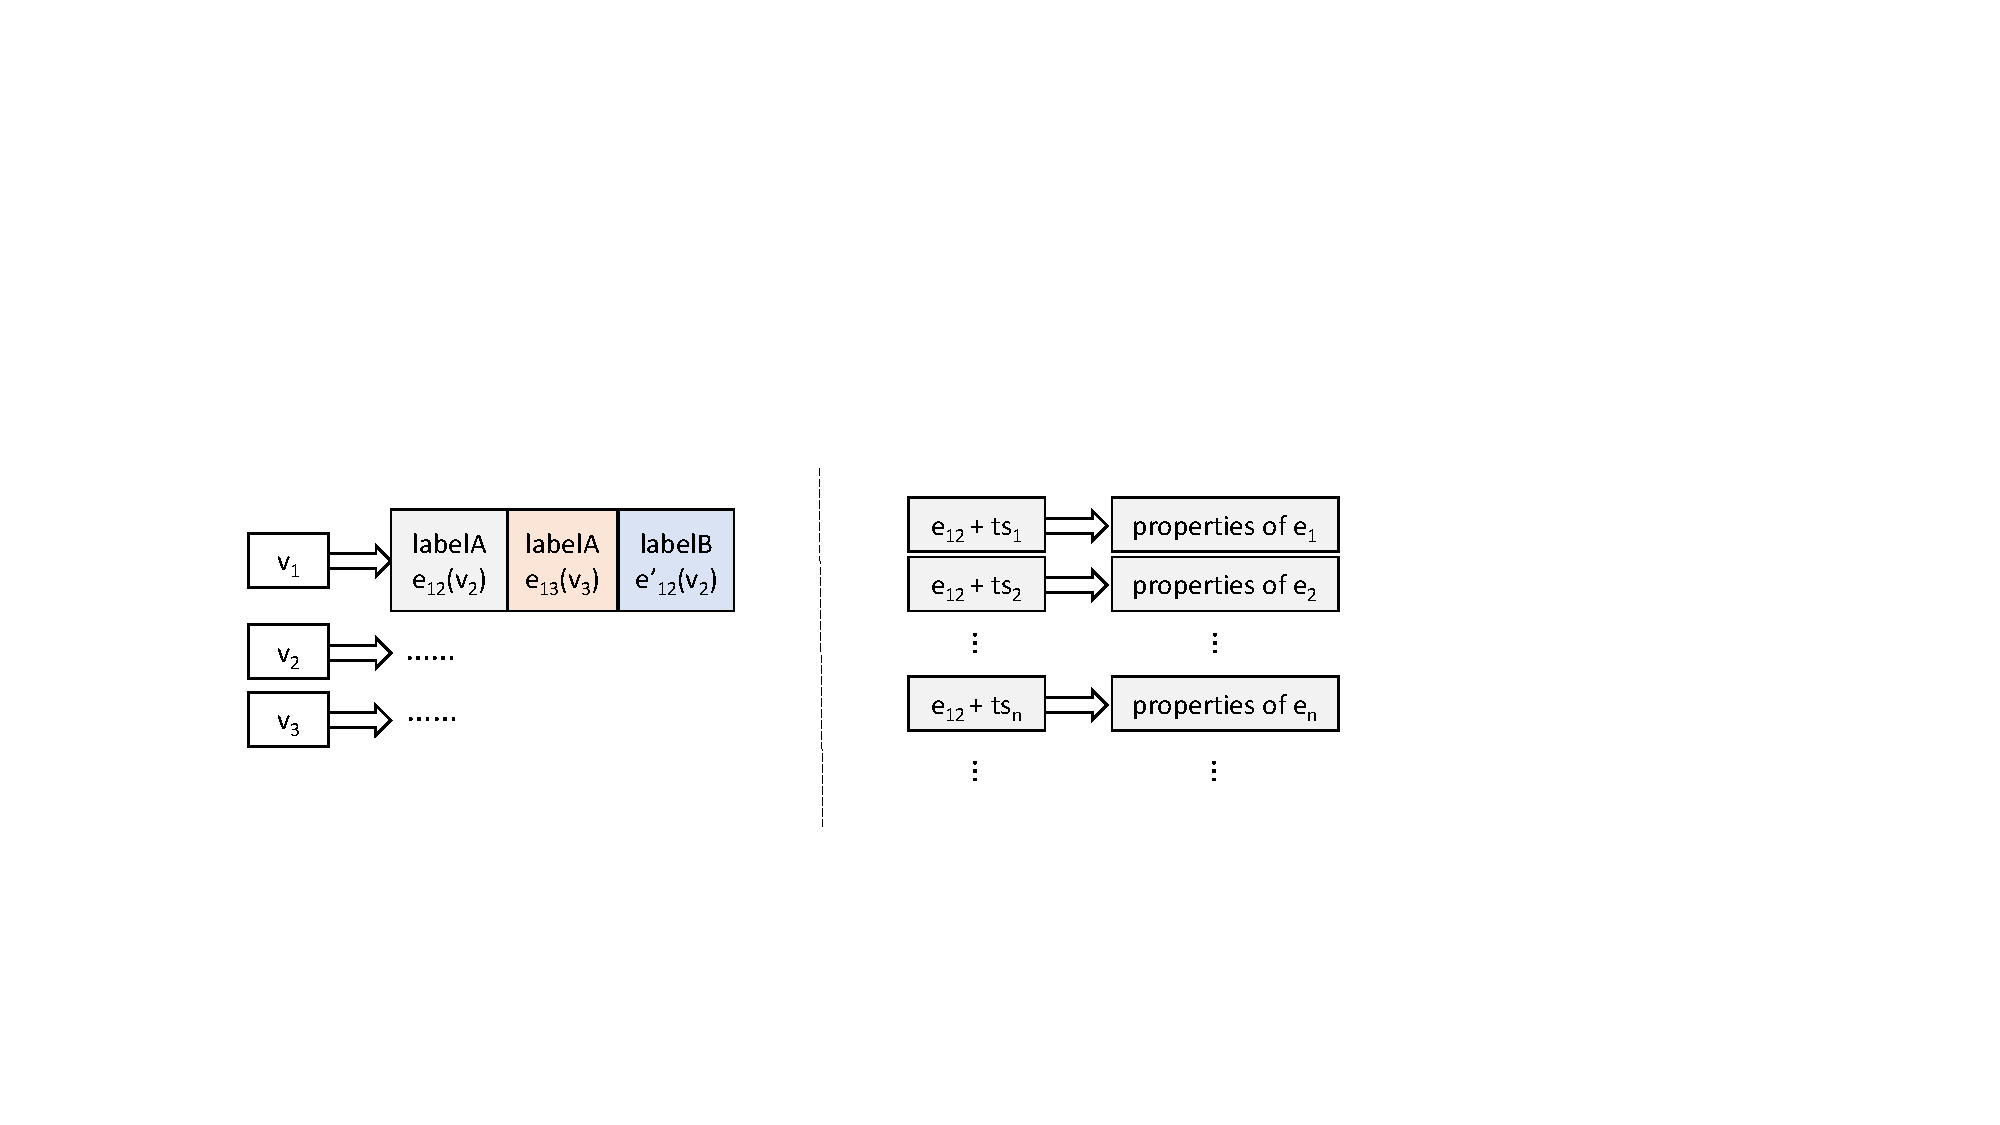
\includegraphics[width=150mm]{fig/curr_list.pdf}
\caption{HybriG在HBase中的数据表分为两张,左边为Titan转化成的数据表,右边为边表。当属性图富含重边时,Titan数据表不被影响,边表将是一张高而窄的表。}
\label{fig:curr_list}
\end{figure}

为了解释HybriG在图查询上的优势,图\ref{fig:curr_list}展示了HybriG在HBase中的表结构,包括Titan自身的HBase数据表和HybriG特殊设计的边表。当属性图的重边数量爆炸性增长时,Titan的数据表并不会被影响,因为两点间同label的边至多只会存在一条,每个点的邻接表列数仍为不同label邻接的点数。另外,Titan中的边只存放统计信息,因此每个单元格(即每条边)的数据量实际很小。面对含有大量重边的属性图,各点的邻接表仍保持了列数和数据量上的精简。即使面对邻域点集查询的全表扫描,也能提供优异的性能。
另一方面,得益于邻接表的精简,Titan的缓存因此可以存放更多点集数据。对于邻域点集相关查询,如多跳邻域(k-hop)查询、路径查询、局部聚集系数计算等,具体的实现往往由多个基本的邻域点集查询组成,缓存的命中率就显得尤为重要。传统的解决方案中使用Titan存储所有的重边,使得缓存中只能存储少量点集的数据,大部分空间被边集数据占据,而具体的边集数据在查询中并不相关。在HybriG架构中,Titan的缓存能充分保留更多的点集数据,从而进一步提高邻域点集相关查询的缓存命中率。
综上,HybriG对邻域点集相关的查询具有很好的表现,后续的实验结果将展示具体的数据。

\subsection{边集相关查询的优势}
在许多刑侦推演场景中,往往只需要查询两点间拥是否拥有某种label的边,而不需要查看具体各个重边的数据。比如得知两人之间有共同住宿酒店的边相连后,基本可以断定两人认识,领域专家可以在图中继续推演出其他相关的人,后续有需要再展开这条关系,查看具体的各条酒店住宿记录。HybriG架构为这种场景提供了便利,上述场景相当于在HybriG架构的Titan图中进行游走(Graph traversal),当有需要时再展开某条边,在HBase边表中读回相应的边数据。
对于边集数据的读取,HybriG将所有边的数据存储在HBase边表中,而且每条边占一行,这使得对边的检索是行级别的检索,即在表中查找一行。传统的解决方案将重边数据都存储在Titan中,边集数据存储于各点的邻接表,而每个点的邻接表在HBase数据表中占据一行,因此对边的检索是选定行后的列级别检索。HBase中行级别的检索要略优于列级别的检索,因此HybriG会略占优势。然而,HybriG对边的检索需要跨Titan和HBase两个系统,会多一次交互的开销。实验表明,这两方面功过相抵,HybriG的边集数据查询性能与Titan相差不大。
HybriG架构在边集统计信息的查询或计算上会有很大优势。在HybriG架构中,Titan中某种label的边存在,代表原属性图中两点间拥有该label的边,具体的重边数据存储在HBase中的边表,而Titan中的边上的则存储了该label声明时设定的统计信息,如具体的重边数目、边上某个属性的最大最小值等。对于这些统计信息,可以直接在Titan中查询得到结果。



% vim:ts=4:sw=4
